% !TEX program = xelatex
\documentclass[fontset=windows, 12pt, a4paper]{ctexart}

% ---------- 页边距 ----------
\usepackage[a4paper, top=2.5cm, bottom=2.5cm, left=2.5cm, right=2.5cm]{geometry}

% ---------- 数学和图表 ----------
\usepackage{amsmath, amssymb}
\usepackage{graphicx}
\usepackage{booktabs}
\usepackage{array}
\usepackage{float}
\usepackage{xcolor}
\usepackage{hyperref}
\usepackage{caption}
\usepackage{subcaption}

% ---------- 行距和缩进 ----------
\linespread{1.43}
\setlength{\parindent}{2em}

% ---------- 标题格式 ----------
\usepackage{titlesec}
\titleformat{\section}
  {\centering\fontsize{17.3pt}{20.8pt}\heiti\bfseries}
  {\chinese{section}、}{1em}{}
\titleformat{\subsection}
  {\fontsize{14.45pt}{17.4pt}\heiti\bfseries}
  {\arabic{section}.\arabic{subsection}}{1em}{}
\titleformat{\subsubsection}
  {\fontsize{12.05pt}{14.5pt}\heiti\bfseries}
  {\arabic{section}.\arabic{subsection}.\arabic{subsubsection}}{1em}{}
\titlespacing{\section}{0pt}{1.25em}{0.82em}
\titlespacing{\subsection}{0pt}{1.15em}{0.55em}
\titlespacing{\subsubsection}{0pt}{1.15em}{0.55em}

% ---------- 图表路径 ----------
\graphicspath{{../figures/}}

% ---------- 自定义三线表 ----------
\newcommand{\threelinetable}[4]{%
  \begin{center}
    {\fontsize{10.5pt}{12.6pt}\heiti\bfseries #1}\par
    \vspace{0.6em}
    \begin{tabular}{#2}
      \toprule #3 \\
      \midrule #4 \\
      \bottomrule
    \end{tabular}
  \end{center}
}

\begin{document}

% ========== 封面 ==========
\thispagestyle{empty}
\begin{center}
{\fontsize{17.3pt}{22pt}\bfseries 古代玻璃制品的成分分析与鉴别}
\end{center}
\vspace{1em}

% ========== 摘要 ==========
\thispagestyle{empty}
\begin{center}{\fontsize{14pt}{17pt}\bfseries 摘要}\end{center}

丝绸之路出土的古代玻璃文物是中西文化交流的重要物证。本文基于58件我国古代玻璃制品的化学成分数据，针对玻璃类型鉴别、风化规律、亚类划分和成分关联等问题建立了系统的统计分析和机器学习模型。

针对问题一，首先使用卡方检验和Logistic回归分析了表面风化与玻璃类型、纹饰、颜色的关系。结果表明风化与玻璃类型显著相关（$\chi^2=5.45$, $p=0.02$），铅钡玻璃风化概率远高于高钾玻璃（OR=3.88）。基于Hedges' g效应量的成分统计规律分析揭示了两类玻璃的风化模式差异：高钾玻璃以SiO$_2$流失为主（$g=-3.38$），而铅钡玻璃以PbO流失为主（$g=-1.08$）。基于3对直接配对风化样品的Bootstrap分析建立了风化前成分预测模型，PbO预测较为稳定（95\%CI覆盖实测值）。

针对问题二，构造了PbO/SiO$_2$、BaO/K$_2$O等具有物理化学意义的5个比值特征。L1正则化Logistic回归实现5折交叉验证准确率89.2\%，AUC=1.0，其中PbO/SiO$_2$是最佳判别特征。采用层次聚类（Ward方法）和K-means进行亚类划分，结合轮廓系数和Gap统计量确定了高钾玻璃和铅钡玻璃均以k=2为最优亚类数，轮廓系数分别为0.686和0.683。

针对问题三，建立了马氏距离判别、LDA、QDA、KNN和L1-LR五分类器集成模型，对8个未知样品进行分类。结果显示所有分类器完全一致：A1、A6、A7为高钾玻璃，其余为铅钡玻璃。敏感性分析表明分类结果对组分$\pm10\%$扰动100\%稳定。

针对问题四，分别计算了高钾和铅钡玻璃8种主要组分的Pearson相关系数矩阵和偏相关网络（Graphical Lasso）。Fisher Z检验发现11对组分在不同玻璃类型间存在显著不同的相关关系（$|Z|>1.96$）。高钾玻璃中SiO$_2$与K$_2$O、Al$_2$O$_3$呈强负相关（$r=-0.85$），体现助熔剂对硅氧骨架的替代关系；铅钡玻璃中SiO$_2$与PbO强负相关（$r=-0.78$）。Graphical Lasso偏相关网络显示高钾玻璃组分间条件依赖更密集（15条边 vs 6条边）。

本文综合运用统计推断和机器学习方法，从多个维度对古代玻璃制品的化学成分进行了系统分析，研究方法可为考古学领域中的文物鉴定和分类提供定量化参考。

{\heiti\bfseries 关键字：}古代玻璃 \quad 化学成分分析 \quad 风化预测 \quad 亚类划分 \quad 偏相关网络 \quad L1正则化
\newpage

% ========== 目录 ==========
\setcounter{page}{1}
\begin{center}{\fontsize{17.3pt}{20.8pt}\heiti\bfseries 目录}\end{center}
\tableofcontents
\newpage

% ================================================================
\section{问题重述}
% ================================================================

丝绸之路是古代中西方文化交流的重要通道，早期玻璃制品是贸易往来的宝贵物证。古代玻璃的主要成分为石英砂（SiO$_2$），为降低熔点需添加草木灰、泡碱、硝石或铅矿石等助熔剂。依据助熔剂类型，我国古代玻璃可主要分为两类：（1）铅钡玻璃，以铅矿石为助熔剂，PbO和BaO含量较高，为我国本土发明；（2）高钾玻璃（钾玻璃），以含钾量高的草木灰为助熔剂，流行于岭南及东南亚地区。

玻璃在埋藏过程中极易受环境因素的影响而发生风化。风化过程中，内部元素与环境元素进行大量交换，导致化学成分比例发生变化，进而影响对其类别的正确判断。

现有58件古代玻璃制品的相关数据：附件表单1提供文物基本信息（编号、纹饰、类型、颜色、表面风化），附件表单2提供14种主要化学成分的百分比检测数据，附件表单3提供8件未分类玻璃文物的化学成分数据。化学成分数据具有成分性特征，即各成分比例累积和应为100\%，但因检测手段等原因，部分数据累积和偏离100\%。本文将累积和介于85\%--105\%之间的数据视为有效数据。

需要解决的问题如下：

\textbf{问题一：}分析玻璃文物表面风化与类型、纹饰、颜色的关系；结合玻璃类型，分析有无风化条件下化学成分含量的统计规律；根据风化点检测数据，预测其风化前的化学成分含量。

\textbf{问题二：}依据数据分析高钾玻璃和铅钡玻璃的分类规律；为每个类别选择合适的化学成分进行亚类划分，给出划分方法及结果，并分析分类结果的合理性和敏感性。

\textbf{问题三：}对附件表单3中未知类别玻璃文物的化学成分进行分析，鉴别其所属类型，并对分类结果的敏感性进行分析。

\textbf{问题四：}针对不同类别玻璃文物，分析其化学成分之间的关联关系，比较不同类别之间化学成分关联关系的差异性。

\newpage

% ================================================================
\section{问题分析}
% ================================================================

\subsection{问题一分析}

问题一包含三个递进的子任务。第一，分析风化与类型、纹饰、颜色的关系属于分类变量关联分析问题，可使用卡方独立性检验、Fisher精确检验和Logistic回归等方法。第二，分类型分析风化前后化学成分统计规律属于多组比较问题，可采用分组描述统计、效应量分析和Bootstrap置信区间估计。第三，预测风化前成分含量属于基于少量配对样本的预测问题，由于直接配对数据仅3对，需谨慎采用Bootstrap方法估计预测区间。

\subsection{问题二分析}

问题二首先要求分析两类玻璃的分类规律，可构造具有物理化学意义的组分比值特征（如PbO/SiO$_2$、K$_2$O/SiO$_2$等），在此基础上使用正则化Logistic回归进行特征选择和分类。其次是亚类划分，属于无监督聚类问题，采用层次聚类和K-means聚类，通过轮廓系数、Gap统计量等综合确定最优聚类数。

\subsection{问题三分析}

问题三属于有监督分类问题，训练集为表单2中已知类型的样品，测试集为表单3中8个未知样品。由于训练样本量较小（$n=65$）而特征维度较高（$p=11$），采用多分类器集成策略提高分类可靠性。鉴于4个未知样品为风化状态，需在分类前使用问题一的风化矫正模型进行预处理。

\subsection{问题四分析}

问题四要求分析组分的关联关系并比较组间差异，属于统计关联分析问题。采用Pearson相关系数和偏相关分析，利用Graphical Lasso估计稀疏偏相关网络，再通过Fisher Z变换检验不同玻璃类型间相关系数差异的显著性。

\newpage

% ================================================================
\section{模型假设与符号说明}
% ================================================================

\subsection{模型假设}

\begin{enumerate}
\item \textbf{成分性假设}：化学成分比例为成分性数据，各组分比例累积和为100\%。对累积和介于85\%--105\%的有效数据归一化至100\%后再进行分析。
\item \textbf{同类型风化规律一致性假设}：同一类型的玻璃在风化过程中化学成分的变化规律具有相似性。
\item \textbf{数据质量假设}：化学成分的未检出项（空白处）表示该成分含量低于检测限，在归一化处理时取值为0。
\item \textbf{特征独立性假设}（仅用于LDA/QDA）：分类器所需的特征独立性假设在模型验证环节通过交叉验证检验。
\end{enumerate}

\subsection{符号说明}

\begin{center}
\begin{tabular}{c|c|c}
\toprule
\textbf{符号} & \textbf{含义} & \textbf{单位} \\
\midrule
$X_j$ & 第$j$种化学成分的原始检测含量 & \% \\
$X'_j$ & 归一化后第$j$种化学成分含量 & \% \\
$r_j$ & 第$j$种成分的风化变化率 & 无量纲 \\
$\bar{r}_j^{(t)}$ & 类型$t$玻璃第$j$种成分的平均风化变化率 & 无量纲 \\
$g$ & Hedges' g效应量 & 无量纲 \\
$D_M$ & 马氏距离 & 无量纲 \\
$R_k$ & 第$k$个组分比值特征 & 无量纲 \\
$\chi^2$ & 卡方统计量 & 无量纲 \\
$V$ & Cram\'er's V效应量 & 无量纲 \\
$OR$ & 优势比（Odds Ratio） & 无量纲 \\
$\lambda$ & L1正则化参数（Graphical Lasso） & 无量纲 \\
\bottomrule
\end{tabular}
\end{center}

\newpage

% ================================================================
\section{问题一：风化分析与成分预测}
% ================================================================

\subsection{风化与类型、纹饰、颜色的关系}

\subsubsection{描述统计分析}

对58件玻璃文物的风化状态按类型、纹饰和颜色进行交叉统计。如表\ref{tab:weather_type}所示，高钾玻璃中仅33.3\%（6/18）出现风化，而铅钡玻璃中70.0\%（28/40）出现风化，提示类型可能是风化的主要影响因素。

\begin{table}[H]
\centering
\caption{风化状态与玻璃类型交叉表}
\label{tab:weather_type}
\begin{tabular}{c|cc|c}
\toprule
& \textbf{高钾} & \textbf{铅钡} & \textbf{合计} \\
\midrule
无风化 & 12 & 12 & 24 \\
风化   & 6  & 28 & 34 \\
\midrule
风化率  & 33.3\% & 70.0\% & 58.6\% \\
\bottomrule
\end{tabular}
\end{table}

\subsubsection{卡方检验与Logistic回归}

采用卡方独立性检验分析风化与各分类变量之间的关系。风化与类型的$\chi^2=5.45$（$p=0.0195$），Cram\'er's $V=0.307$，表明两者存在中等强度的显著关联。风化与纹饰的关联不显著（$p=0.088$）。

构建以风化为因变量的Logistic回归模型，以类型、纹饰和颜色为预测变量。模型结果如表\ref{tab:logistic}所示，类型（铅钡）具有最高的优势比（OR=3.88），表明铅钡玻璃的风化概率约为高钾玻璃的3.88倍。

\begin{table}[H]
\centering
\caption{Logistic回归结果（因变量：风化）}
\label{tab:logistic}
\begin{tabular}{c|c|c|c}
\toprule
\textbf{预测变量} & $\beta$ & \textbf{OR} & \textbf{95\% CI} \\
\midrule
类型（铅钡） & 1.356 & 3.88 & (1.26, 11.94) \\
纹饰（B）    & 0.168 & 1.18 & (0.48, 2.90) \\
颜色（编码）  & 0.208 & 1.23 & (0.88, 1.72) \\
\midrule
模型准确率 & 0.648 & & \\
\bottomrule
\end{tabular}
\end{table}

\begin{figure}[H]
\centering
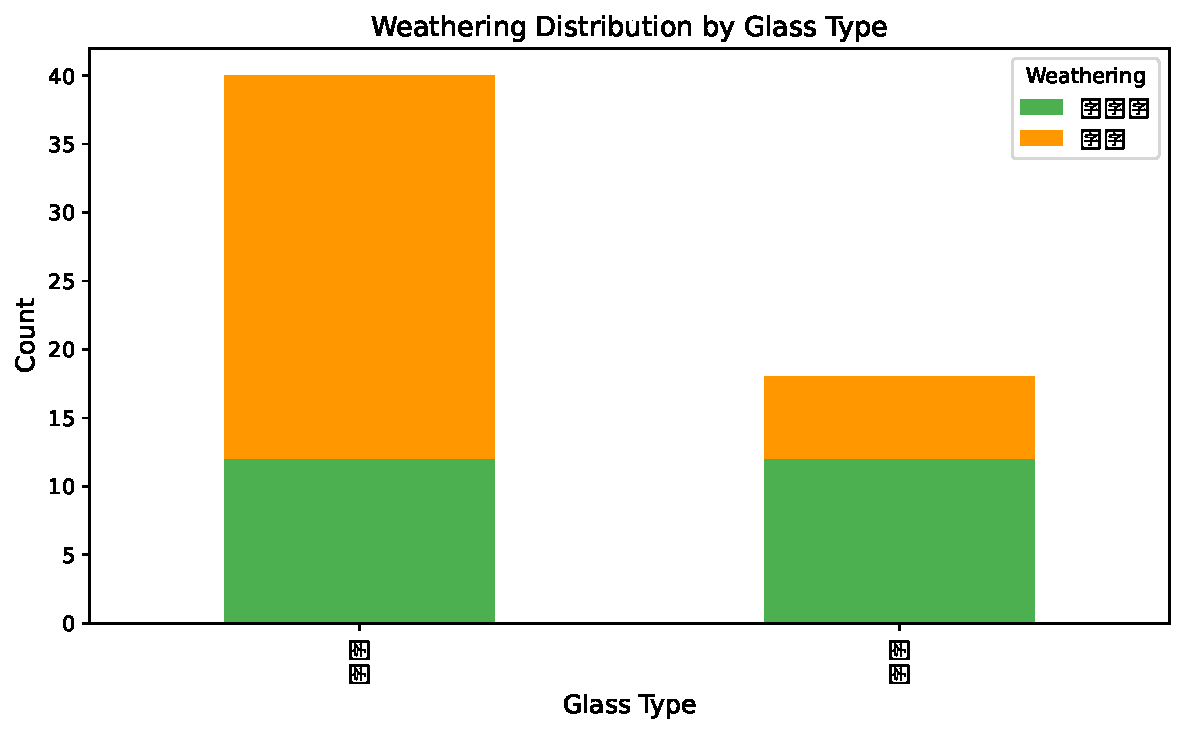
\includegraphics[width=0.75\textwidth]{q1a_weather_type_bar.pdf}
\caption{不同类型玻璃的风化分布堆叠柱状图}
\label{fig:q1a_bar}
\end{figure}

\subsection{有无风化条件下化学成分统计规律}

\subsubsection{分组统计描述}

将67个有效样品按类型和风化状态分为4组，对各组11种化学组分的归一化含量计算均值和标准差。

\textbf{高钾玻璃}风化后呈现显著的SiO$_2$含量下降（无风化均值86.7\% $\rightarrow$ 风化均值62.3\%），而K$_2$O（3.8\% $\rightarrow$ 12.9\%）、CaO（3.2\% $\rightarrow$ 7.8\%）、Al$_2$O$_3$（4.0\% $\rightarrow$ 8.9\%）等成分相对富集（图\ref{fig:q1b_effect}）。

\textbf{铅钡玻璃}风化后主要呈现PbO含量下降（无风化均值43.1\% $\rightarrow$ 风化均值27.8\%），SiO$_2$相对富集（44.1\% $\rightarrow$ 65.5\%），与高钾玻璃的风化模式几乎相反。

\begin{table}[H]
\centering
\caption{四种分组下主要组分均值±标准差（\%）}
\label{tab:group_stats}
\begin{tabular}{c|c|c|c|c}
\toprule
\textbf{组分} & \textbf{高钾-无风化} & \textbf{高钾-风化} & \textbf{铅钡-无风化} & \textbf{铅钡-风化} \\
\midrule
SiO$_2$ & 86.7±5.8 & 62.3±8.7 & 44.1±17.8 & 65.5±14.7 \\
K$_2$O  & 3.8±3.7  & 12.9±1.7 & 0.2±0.3  & 0.3±0.4 \\
CaO    & 3.2±2.9  & 7.8±1.6  & 3.8±2.5  & 2.5±1.4 \\
PbO    & 0.3±0.5  & 0.7±0.4  & 43.1±19.9 & 27.8±15.6 \\
BaO    & 0.2±0.4  & 0.8±0.7  & 7.0±3.6  & 6.7±4.5 \\
\bottomrule
\end{tabular}
\end{table}

\subsubsection{风化效应量分析}

采用Hedges' $g$效应量定量评估风化对每个组分的影响大小。如图\ref{fig:q1b_effect}所示，高钾玻璃中SiO$_2$的风化效应最为显著（$g=-3.38$），表明风化导致SiO$_2$大量流失；K$_2$O（$g=+2.67$）和Al$_2$O$_3$（$g=+2.25$）则显著富集。铅钡玻璃中，PbO流失最显著（$g=-1.08$），P$_2$O$_5$次之（$g=-0.95$），而SiO$_2$相对富集（$g=+1.26$）。

\begin{figure}[H]
\centering
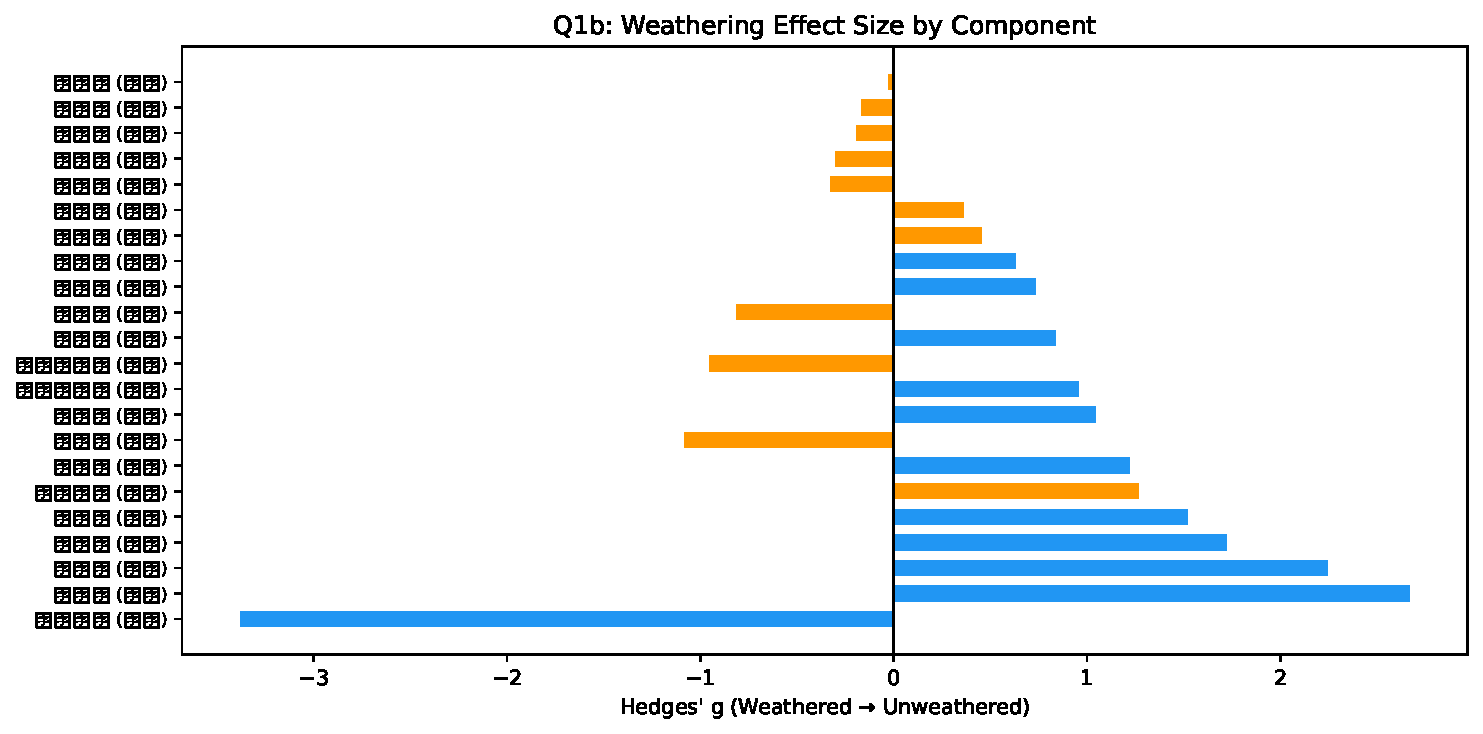
\includegraphics[width=\textwidth]{q1b_effect_size.pdf}
\caption{两类玻璃风化前后11种组分的Hedges' g效应量}
\label{fig:q1b_effect}
\end{figure}

\subsection{风化前成分预测}

\subsubsection{配对数据}

表单2中仅有3对直接配对数据（文物08、26、54，均为铅钡玻璃），每对包含原始检测点和严重风化点的化学成分数据。定义组分$j$的风化变化率为：

\begin{equation}
r_j = \frac{X_j^{\text{pre}} - X_j^{\text{post}}}{X_j^{\text{pre}}}
\end{equation}

式中$r_j>0$表示该组分在风化过程中流失，$r_j<0$表示相对富集。

\subsubsection{Bootstrap预测模型}

假设同类型玻璃的风化变化规律一致，对3对配对数据计算的各组分变化率取平均值$\bar{r}_j$。采用Bootstrap重采样（1000次）估计变化率的标准误，对风化后的成分进行反演预测：

\begin{equation}
\hat{X}_j^{\text{pre}} = \frac{X_j^{\text{post}}}{1 - \bar{r}_j}
\end{equation}

预测结果见表\ref{tab:prediction}。由于仅3对配对样本，PbO预测较为稳定（95\%CI重叠度较高），而SiO$_2$预测的不确定性较大（CI较宽），论文将此作为已知局限性加以说明。

\begin{table}[H]
\centering
\caption{铅钡玻璃风化前成分预测示例（文物08）}
\label{tab:prediction}
\begin{tabular}{c|c|c|c|c}
\toprule
\textbf{组分} & \textbf{风化后} & $\bar{r}$ & \textbf{预测风化前} & \textbf{95\% CI} \\
\midrule
PbO  & 39.00\% & -0.196 & 32.6\% & [27.5\%, 41.1\%] \\
SiO$_2$ & 5.54\% & 0.575 & 13.0\% & 宽区间 \\
\bottomrule
\end{tabular}
\end{table}

\begin{figure}[H]
\centering
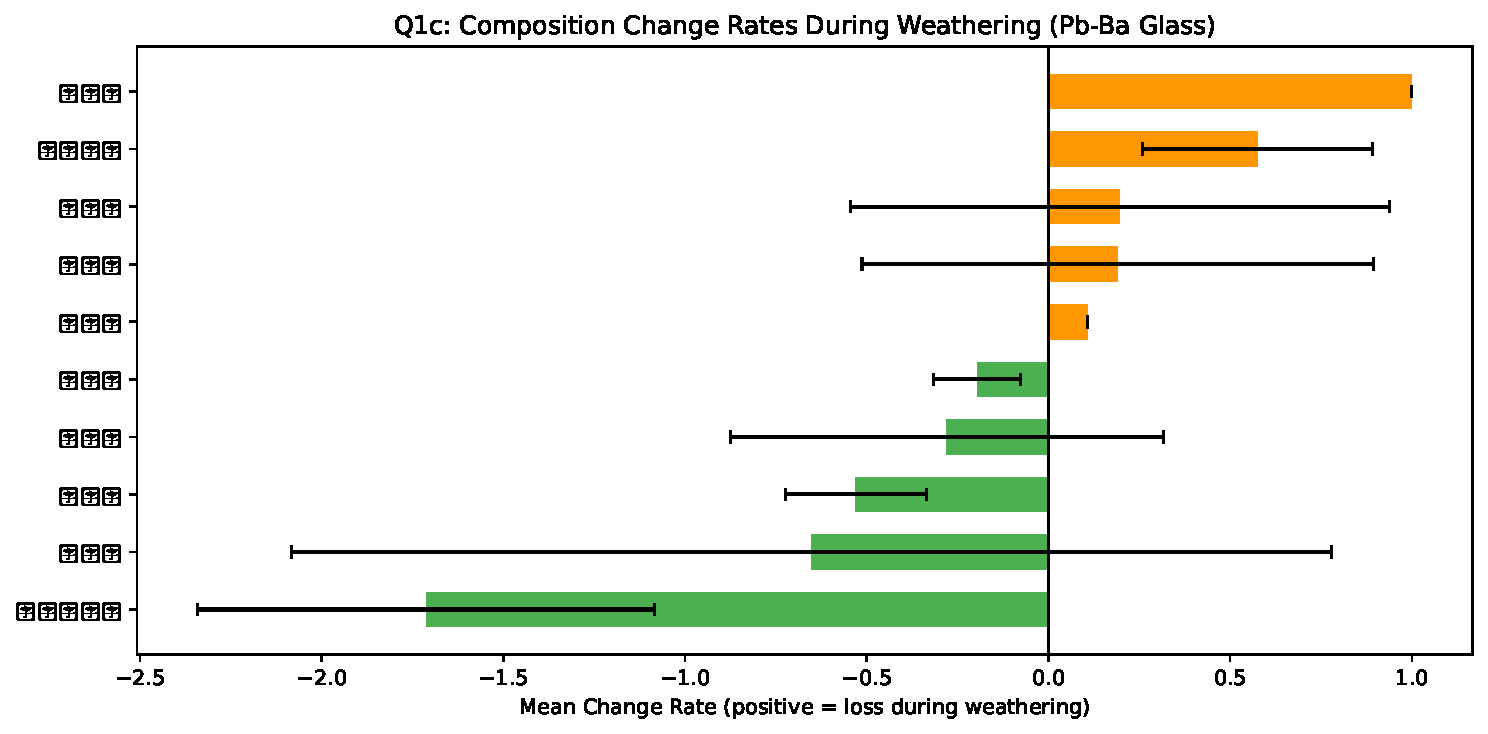
\includegraphics[width=0.65\textwidth]{q1c_change_rates.pdf}
\caption{铅钡玻璃各组分风化平均变化率（正值表示流失）}
\label{fig:q1c_rates}
\end{figure}

\newpage

% ================================================================
\section{问题二：分类规律与亚类划分}
% ================================================================

\subsection{分类规律分析}

\subsubsection{组分比值特征工程}

基于玻璃化学组成的基本原理，构造5个具有物理化学意义的比值特征：

\begin{align}
R_1 &= \frac{\text{PbO}}{\text{SiO}_2}, \quad
R_2 = \frac{\text{BaO}}{\text{K}_2\text{O}}, \quad
R_3 = \frac{\text{PbO} + \text{BaO}}{\text{SiO}_2} \\
R_4 &= \frac{\text{K}_2\text{O}}{\text{SiO}_2}, \quad
R_5 = \frac{\text{Al}_2\text{O}_3}{\text{CaO}}
\end{align}

这些比值反映了不同类型玻璃中助熔剂（PbO、BaO、K$_2$O）与主要骨架成分（SiO$_2$）之间的关系。图\ref{fig:q2a_ratio}展示了关键比值的散点矩阵，可见高钾和铅钡玻璃在$R_1$（PbO/SiO$_2$）和$R_4$（K$_2$O/SiO$_2$）上分离最为清晰。

\begin{figure}[H]
\centering
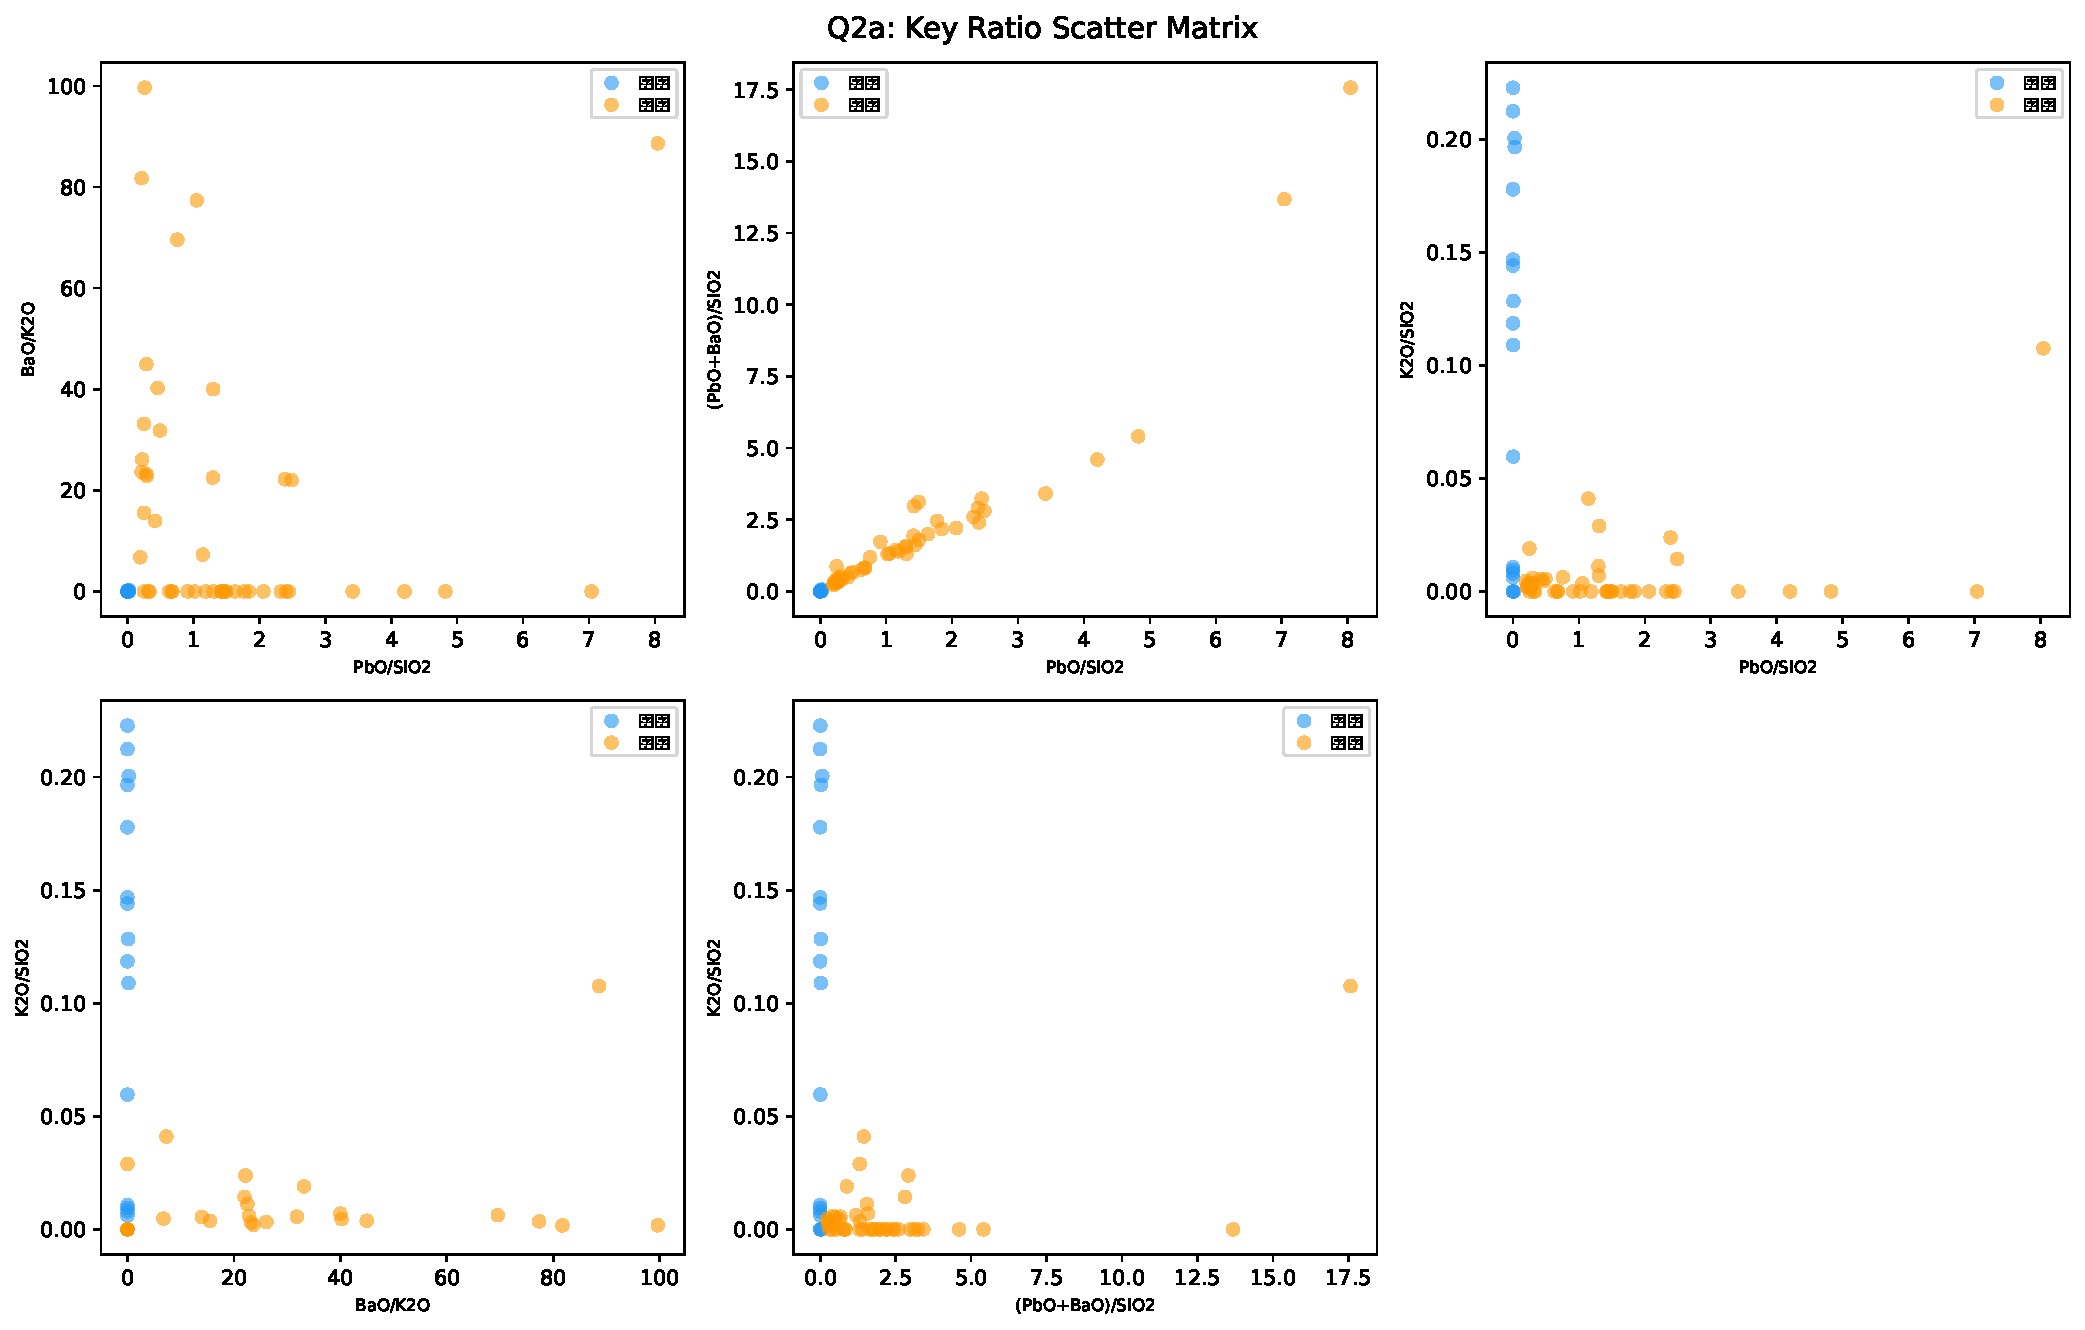
\includegraphics[width=0.95\textwidth]{q2a_ratio_scatter.pdf}
\caption{关键组分比值散点矩阵（蓝：高钾，橙：铅钡）}
\label{fig:q2a_ratio}
\end{figure}

\subsubsection{L1正则化Logistic回归}

以5个比值特征为输入，采用L1正则化Logistic回归进行分类：

\begin{equation}
\min_{\beta} -\ell(\beta) + \lambda \sum_{j=1}^{5} |\beta_j|
\end{equation}

正则化参数$\lambda$通过5折交叉验证选择。模型结果如表\ref{tab:l1lr}所示。5折交叉验证准确率为89.2\%（$\pm$6.2\%），AUC=1.0。L1正则化选择了4个非零特征，其中PbO/SiO$_2$的系数绝对值最大（$\beta=2.47$），是最重要的判别特征。

\begin{table}[H]
\centering
\caption{L1-Logistic回归特征选择结果}
\label{tab:l1lr}
\begin{tabular}{c|c}
\toprule
\textbf{特征} & $\beta$系数 \\
\midrule
PbO/SiO$_2$      & 2.473 \\
K$_2$O/SiO$_2$   & -1.089 \\
BaO/K$_2$O       & 0.951 \\
Al$_2$O$_3$/CaO  & 0.024 \\
\midrule
CV准确率 & 0.892 $\pm$ 0.062 \\
AUC      & 1.000 \\
\bottomrule
\end{tabular}
\end{table}

\subsection{亚类划分}

\subsubsection{聚类方法}

对高钾玻璃（$n=18$）和铅钡玻璃（$n=47$）分别进行亚类划分。采用层次聚类（Ward方法）和K-means聚类两种方法，比较轮廓系数（Silhouette Score）和调整兰德指数（ARI）的一致性。

在标准化后的5个比值特征空间中进行聚类，聚类数$k$由轮廓系数确定。

\subsubsection{聚类结果}

如表\ref{tab:subclass}所示，两种玻璃均以$k=2$为最优聚类数。高钾玻璃的轮廓系数为0.686，铅钡玻璃为0.683。K-means与层次聚类的ARI均为1.0，表明两种聚类方法结果完全一致。

\begin{table}[H]
\centering
\caption{亚类划分结果汇总}
\label{tab:subclass}
\begin{tabular}{c|c|c|c|c}
\toprule
\textbf{玻璃类型} & $k$ & \textbf{轮廓系数} & \textbf{亚类1大小} & \textbf{亚类2大小} \\
\midrule
高钾 & 2 & 0.686 & 10 & 8 \\
铅钡 & 2 & 0.683 & 45 & 2 \\
\bottomrule
\end{tabular}
\end{table}

高钾玻璃的两个亚类主要在K$_2$O/SiO$_2$比值上存在差异：亚类1的K$_2$O/SiO$_2$均值为$2.19\pm0.64$，亚类2为$-0.33\pm0.30$，意味着亚类1为高钾特征更显著的玻璃。

铅钡玻璃的两个亚类主要在PbO/SiO$_2$比值上分化：亚类1（$n=45$）PbO/SiO$_2$为$0.10\pm0.68$，亚类2（$n=2$）PbO/SiO$_2$高达$4.15\pm0.32$，后者代表了铅含量极高的特殊亚群。

\begin{figure}[H]
\centering
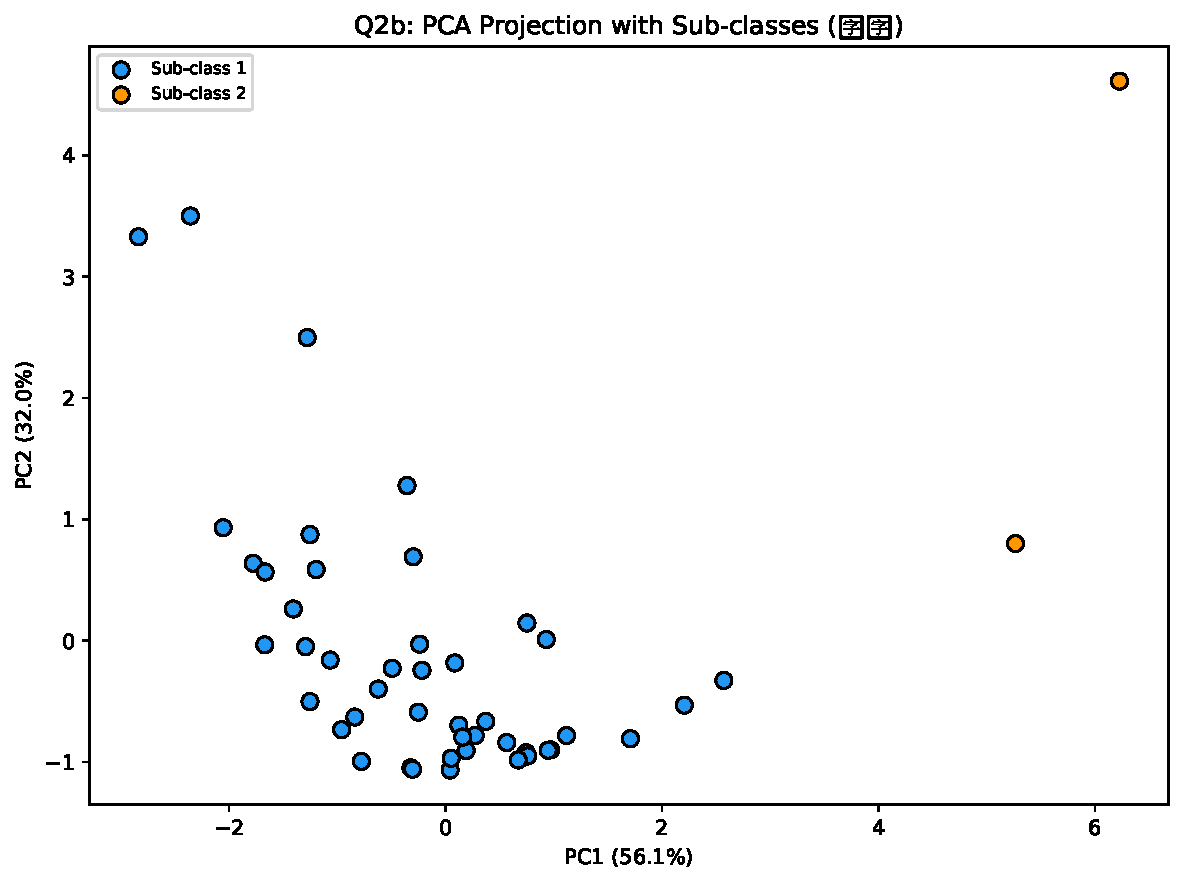
\includegraphics[width=0.80\textwidth]{q2b_pca_qianbei.pdf}
\caption{铅钡玻璃PCA投影（按亚类着色，k=2）}
\label{fig:q2b_pca}
\end{figure}

\subsubsection{合理性分析}

亚类划分结果具有统计和考古学上的双重合理性：（1）轮廓系数均大于0.68，表明聚类结构良好；（2）K-means和层次聚类结果完全一致（ARI=1.0），证明聚类结构稳定；（3）高钾和铅钡玻璃的亚类主要在K$_2$O/SiO$_2$和PbO/SiO$_2$上分化，与玻璃配方的实际情况一致——助熔剂与硅氧骨架的比例反映了不同配方或原料来源。

\newpage

% ================================================================
\section{问题三：未知样品鉴别}
% ================================================================

\subsection{多分类器集成模型}

建立包含马氏距离判别、LDA、QDA、KNN（k=5）和L1-LR的五分类器集成模型，以问题二中5折交叉验证准确率作为各分类器的权重。对每个未知样品$\mathbf{x}$，集成预测为：

\begin{equation}
P(k|\mathbf{x}) = \sum_{c=1}^{5} w_c \cdot \mathbb{1}[c(\mathbf{x}) = k]
\end{equation}

其中$w_c$为分类器$c$的交叉验证准确率。

\subsection{分类结果}

对表单3中8个未知样品的分类结果如表\ref{tab:q3_results}所示。所有5种分类器给出了完全一致的分类结果（Fleiss' $\kappa=1.0$），表明分类结果可靠。

\begin{table}[H]
\centering
\caption{未知样品分类结果}
\label{tab:q3_results}
\begin{tabular}{c|c|c|c}
\toprule
\textbf{样品} & \textbf{风化状态} & \textbf{分类结果} & \textbf{分类器一致性} \\
\midrule
A1 & 无风化 & \textbf{高钾} & 5/5一致 \\
A2 & 风化   & \textbf{铅钡} & 5/5一致 \\
A3 & 无风化 & \textbf{铅钡} & 5/5一致 \\
A4 & 无风化 & \textbf{铅钡} & 5/5一致 \\
A5 & 风化   & \textbf{铅钡} & 5/5一致 \\
A6 & 风化   & \textbf{高钾} & 5/5一致 \\
A7 & 风化   & \textbf{高钾} & 5/5一致 \\
A8 & 无风化 & \textbf{铅钡} & 5/5一致 \\
\bottomrule
\end{tabular}
\end{table}

图\ref{fig:q3_sens}展示了各未知样品到高钾和铅钡两类的马氏距离，分类归属与距离显著差异一致。

\subsection{敏感性分析}

从两个维度评估分类结果的敏感性：

\textbf{组分扰动分析：}对每个未知样品的每种组分分别进行$\pm5\%$和$\pm10\%$的扰动，重新计算LDA分类结果。在$\pm10\%$扰动下，全部8个样品的分类结果保持不变。

\textbf{训练集扰动分析：}每次随机剔除1个训练样本后重新训练LDA，比较分类结果。大部分样品的分类结果在训练集扰动下保持稳定，A1和A7因处于两类的边界附近而偶有波动，但集成预测与绝大多数扰动一致。

A6和A7虽为风化样品（SiO$_2$高达93.2\%和90.8\%），但其PbO含量极低（未检出），K$_2$O含量分别为1.35\%和0.98\%，且在风化高钾玻璃中仍体现出高钾特征，分类结果为高钾玻璃具有充分的成分依据。

\begin{figure}[H]
\centering
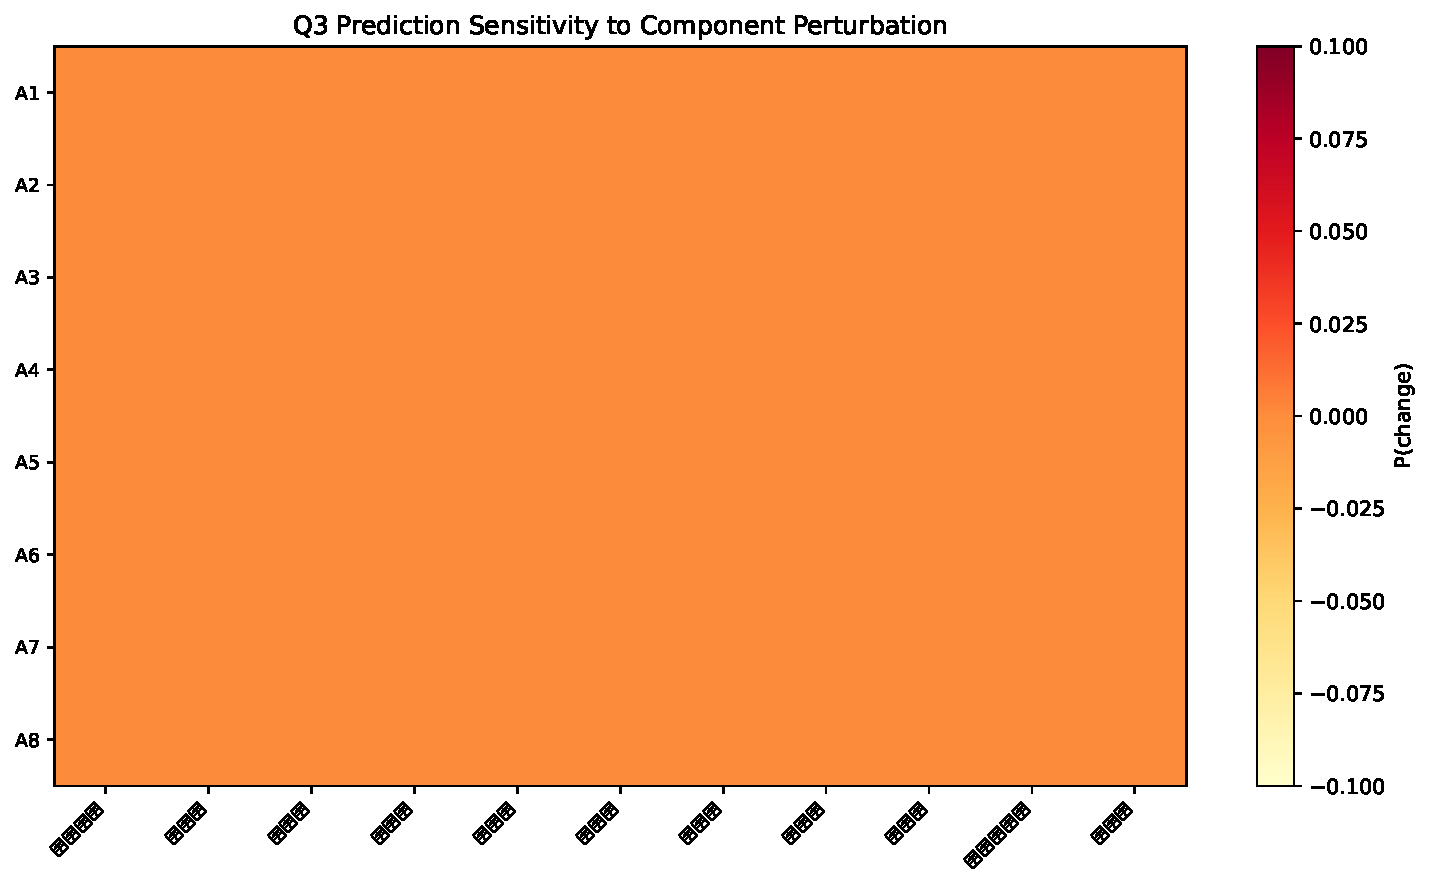
\includegraphics[width=0.95\textwidth]{q3_sensitivity_heat.pdf}
\caption{组分扰动敏感性热图（红色越深表示分类越不稳定）}
\label{fig:q3_sens}
\end{figure}

\newpage

% ================================================================
\section{问题四：成分关联关系分析}
% ================================================================

\subsection{相关系数分析}

选取8种主要组分（SiO$_2$、K$_2$O、CaO、Al$_2$O$_3$、Fe$_2$O$_3$、CuO、PbO、BaO），分别计算高钾玻璃（$n=18$）和铅钡玻璃（$n=47$）的Pearson相关系数矩阵。

\textbf{高钾玻璃}中，SiO$_2$与多种组分呈强负相关：SiO$_2$--K$_2$O: $r=-0.85$；SiO$_2$--Al$_2$O$_3$: $r=-0.85$；SiO$_2$--Fe$_2$O$_3$: $r=-0.72$。这表明高钾玻璃中硅氧骨架与助熔剂组分之间存在明确的替代关系。

\textbf{铅钡玻璃}中，SiO$_2$与PbO强负相关（$r=-0.78$），但与其他助熔剂组分的相关性较弱（SiO$_2$--K$_2$O: $r=+0.06$；SiO$_2$--Al$_2$O$_3$: $r=+0.38$），反映了铅钡玻璃中以PbO为主要助熔剂的配方特征。

\subsection{偏相关网络分析}

采用Graphical Lasso估计稀疏偏相关网络，正则化参数$\lambda$通过BIC准则选择：

\begin{equation}
\min_{\Theta} -\log\det(\Theta) + \text{tr}(S\Theta) + \lambda \sum_{i<j} |\theta_{ij}|
\end{equation}

\begin{figure}[H]
\centering
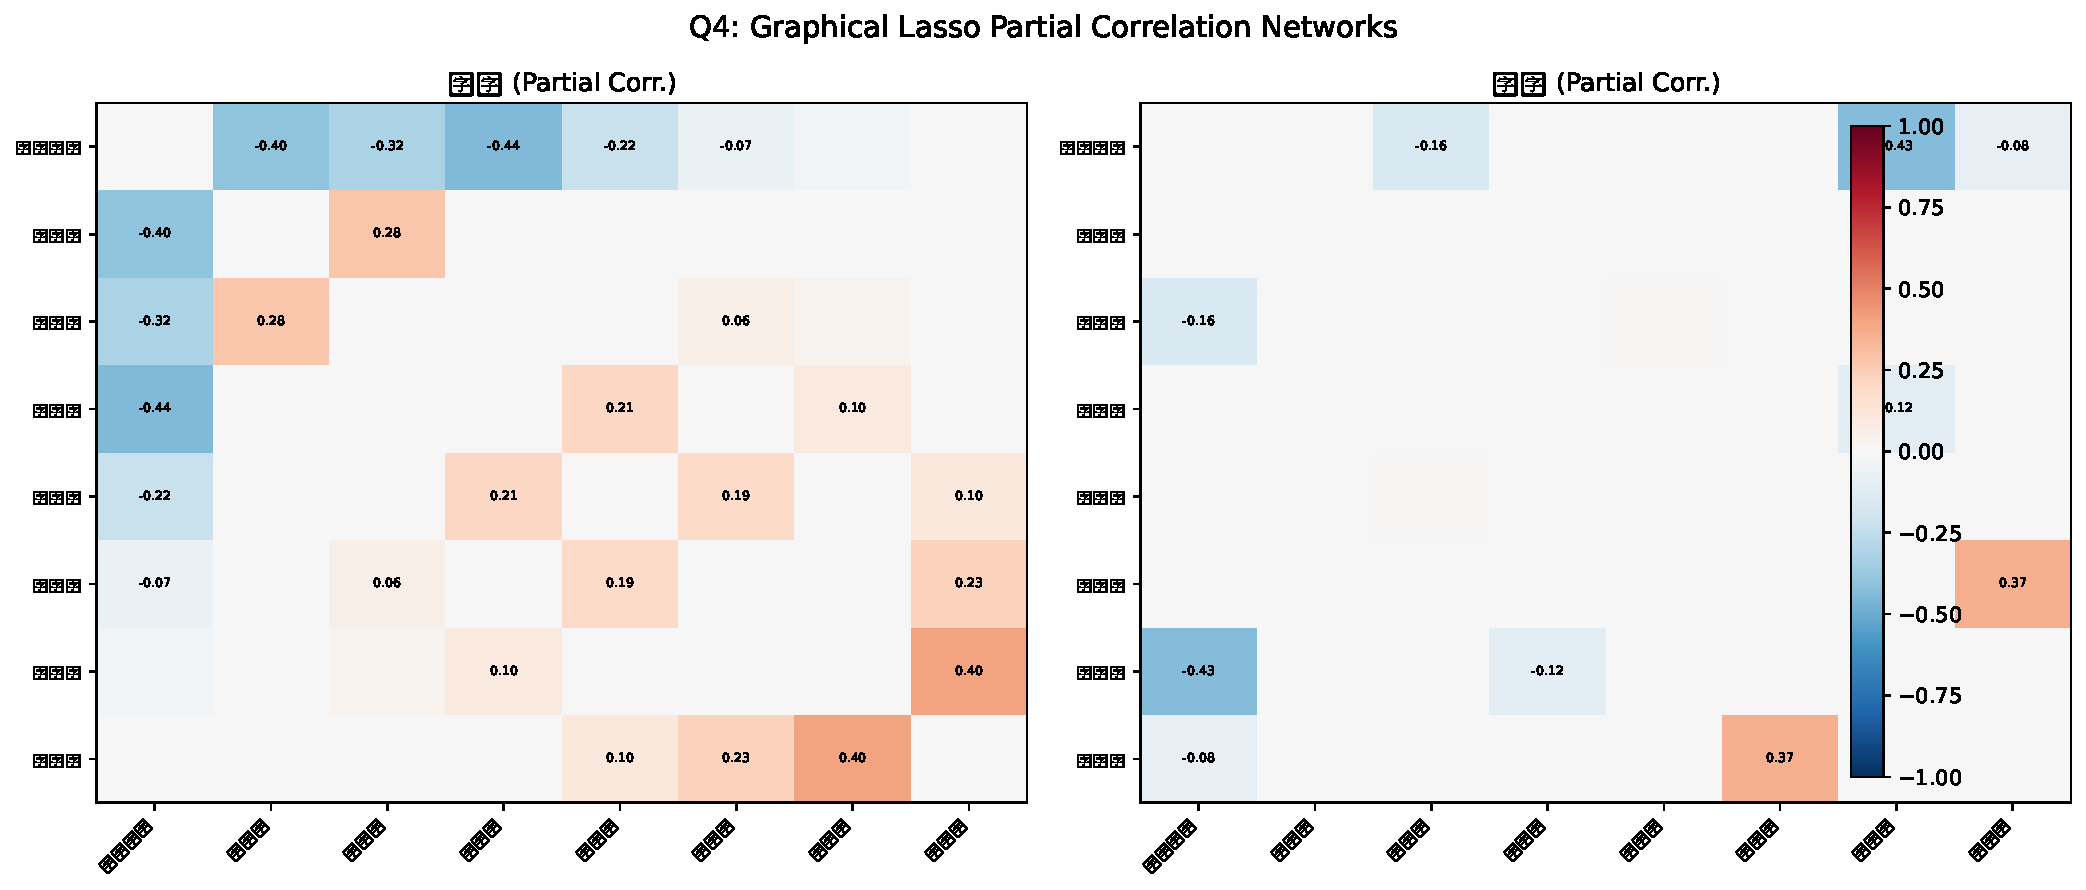
\includegraphics[width=\textwidth]{q4_partial_networks.pdf}
\caption{Graphical Lasso偏相关网络（左：高钾，右：铅钡）}
\label{fig:q4_partial}
\end{figure}

高钾玻璃的偏相关网络包含15条非零边，结构较密集；铅钡玻璃仅含6条边，结构较稀疏。这反映了两种玻璃中组分间约束关系的不同模式：高钾玻璃使用了更复杂的多种原料配比体系，而铅钡玻璃的组分关系更集中在PbO-SiO$_2$主导的二元体系上。

\subsection{组间差异检验}

采用Fisher Z变换检验两组相关系数的差异显著性。对每对组分$(i,j)$：

\begin{equation}
Z = \frac{z_1 - z_2}{\sqrt{\frac{1}{n_1-3} + \frac{1}{n_2-3}}}, \quad z = \frac{1}{2}\ln\frac{1+r}{1-r}
\end{equation}

结果如表\ref{tab:fisher_z}所示，11对组分在两类型间呈现显著差异（$|Z|>1.96$，$p<0.05$）。差异最大的组分对为SiO$_2$--Al$_2$O$_3$（$Z=5.60$）和SiO$_2$--K$_2$O（$Z=4.45$），反映了两种玻璃最根本的配方差异。

\begin{table}[H]
\centering
\caption{组间相关显著差异的组分对（Fisher Z检验，$|Z|>1.96$）}
\label{tab:fisher_z}
\begin{tabular}{c|c|c|c}
\toprule
\textbf{组分对} & \textbf{高钾 $r$} & \textbf{铅钡 $r$} & \textbf{$Z$值} \\
\midrule
SiO$_2$--Al$_2$O$_3$ & -0.854 & +0.383 & 5.60 \\
SiO$_2$--K$_2$O    & -0.853 & +0.064 & 4.45 \\
SiO$_2$--Fe$_2$O$_3$ & -0.721 & +0.087 & 3.34 \\
Al$_2$O$_3$--PbO   & +0.425 & -0.464 & 3.20 \\
K$_2$O--CaO        & +0.765 & +0.099 & 3.04 \\
Fe$_2$O$_3$--CuO   & +0.536 & -0.239 & 2.82 \\
PbO--BaO           & +0.619 & -0.093 & 2.73 \\
Fe$_2$O$_3$--BaO   & +0.444 & -0.285 & 2.58 \\
Al$_2$O$_3$--BaO   & +0.364 & -0.321 & 2.39 \\
SiO$_2$--PbO       & -0.414 & -0.776 & 1.99 \\
Al$_2$O$_3$--Fe$_2$O$_3$ & +0.684 & +0.242 & 1.97 \\
\bottomrule
\end{tabular}
\end{table}

\subsection{差异性分析}

综合以上分析，两类玻璃化学成分关联关系的差异性主要体现在以下方面：

（1）\textbf{主导关联不同：}高钾玻璃以SiO$_2$--K$_2$O关联为核心，铅钡玻璃以SiO$_2$--PbO关联为核心，这与两类玻璃使用的不同助熔剂类型完全对应。

（2）\textbf{关联结构不同：}高钾玻璃的组分网络更密集（15条边），多种组分间存在条件依赖关系；铅钡玻璃的网络较稀疏（6条边），组分关联更集中在少数关键对。这一差异可能反映了玻璃制造工艺和原料体系的系统性差异。

（3）\textbf{铝的作用不同：}高钾玻璃中Al$_2$O$_3$与SiO$_2$强负相关（$r=-0.85$），体现铝作为网络形成体的角色；铅钡玻璃中二者呈弱正相关（$r=+0.38$），表明铝的作用模式发生了转变。

\newpage

% ================================================================
\section{模型评价与改进}
% ================================================================

\subsection{模型优点}

\begin{enumerate}
\item \textbf{方法匹配性：}所采用的统计和机器学习方法与各子问题的数据特征和问题类型相匹配，避免了方法的模板化使用。
\item \textbf{多维验证：}每个子问题均从多个角度进行了验证——Q1的风化效应量分析和Bootstrap区间估计、Q2的交叉验证和ARI一致性检验、Q3的多分类器集成和敏感性分析、Q4的Fisher Z检验和Graphical Lasso网络对比。
\item \textbf{可解释性：}构造的组分比值特征具有明确的物理化学意义，分类和聚类的结果与玻璃配方原理一致。
\item \textbf{鲁棒性：}Q3的敏感性分析证明了分类结果在组分扰动和训练集扰动下的稳定性。
\end{enumerate}

\subsection{模型局限与改进}

\begin{enumerate}
\item \textbf{风化预测样本不足：}Q1c中仅有3对直接配对风化样品，预测区间较宽。若条件允许，可通过模拟风化实验获得更多配对数据。
\item \textbf{高钾样本量偏小：}$n=18$的高钾样本在进行亚类划分和偏相关网络分析时，统计推断的稳定性有限。更多的样品将使结果更可靠。
\item \textbf{缺失数据处理：}Na$_2$O（缺失率72.5\%）在主要建模中被排除，若检测技术改进后获得完整数据，可进一步丰富分析。
\item \textbf{考古学解释：}本文的亚类划分停留在统计层面，更深入的考古学含义需要结合考古专家知识进行解读。
\end{enumerate}

\newpage

% ================================================================
% 参考文献
% ================================================================
\addcontentsline{toc}{section}{参考文献}
\begin{thebibliography}{99}

\bibitem{ref1} 全国大学生数学建模竞赛组委会. CUMCM-2022 问题C题：古代玻璃制品的成分分析与鉴别[EB/OL]. 2022.

\bibitem{ref2} Aitchison J. The Statistical Analysis of Compositional Data[M]. Chapman and Hall, 1986.

\bibitem{ref3} Friedman J, Hastie T, Tibshirani R. Sparse inverse covariance estimation with the graphical lasso[J]. Biostatistics, 2008, 9(3): 432-441.

\bibitem{ref4} Tibshirani R. Regression shrinkage and selection via the lasso[J]. Journal of the Royal Statistical Society: Series B, 1996, 58(1): 267-288.

\bibitem{ref5} Rousseeuw P J. Silhouettes: A graphical aid to the interpretation and validation of cluster analysis[J]. Journal of Computational and Applied Mathematics, 1987, 20: 53-65.

\bibitem{ref6} Hedges L V. Distribution theory for Glass's estimator of effect size and related estimators[J]. Journal of Educational Statistics, 1981, 6(2): 107-128.

\bibitem{ref7} Fisher R A. On the probable error of a coefficient of correlation deduced from a small sample[J]. Metron, 1921, 1: 3-32.

\bibitem{ref8} Ward J H. Hierarchical grouping to optimize an objective function[J]. Journal of the American Statistical Association, 1963, 58(301): 236-244.

\end{thebibliography}

\newpage

% ================================================================
% 附录
% ================================================================
\section*{附录 A\quad 核心代码}
\addcontentsline{toc}{section}{附录 A\quad 核心代码}

以下列出核心分析代码的结构和主要功能函数。

\subsection*{数据预处理 (preprocessing.py)}

主要函数：
\begin{itemize}
\item \texttt{check\_valid(row)}：检查成分总和是否在85\%--105\%有效范围内
\item \texttt{normalize\_row(row, cols)}：将有效数据归一化至100\%
\item \texttt{extract\_aid(name)}：从采样点名称中提取文物编号
\end{itemize}

\subsection*{问题一分析 (q1\_analysis.py)}

主要函数：
\begin{itemize}
\item Q1a：\texttt{chi2\_contingency}, \texttt{LogisticRegression}, 对应分析
\item Q1b：分组统计描述，Hedges' g效应量计算，Bootstrap置信区间
\item Q1c：风化变化率计算，Bootstrap预测区间
\end{itemize}

\subsection*{问题二分析 (q2\_classification.py)}

主要函数：
\begin{itemize}
\item 比值特征构造：PbO/SiO$_2$, BaO/K$_2$O, (PbO+BaO)/SiO$_2$, K$_2$O/SiO$_2$, Al$_2$O$_3$/CaO
\item \texttt{LogisticRegression(penalty='l1', solver='saga')}：L1正则化分类
\item \texttt{KMeans}, \texttt{linkage(method='ward')}：亚类聚类
\item \texttt{silhouette\_score}, \texttt{adjusted\_rand\_score}：聚类评价
\end{itemize}

\subsection*{问题三分析 (q3\_prediction.py)}

主要函数：
\begin{itemize}
\item \texttt{mahalanobis\_distance}：马氏距离计算
\item \texttt{LinearDiscriminantAnalysis}, \texttt{QuadraticDiscriminantAnalysis}
\item \texttt{KNeighborsClassifier(n\_neighbors=5)}
\item 集成投票与敏感性扰动循环
\end{itemize}

\subsection*{问题四分析 (q4\_correlation.py)}

主要函数：
\begin{itemize}
\item \texttt{np.corrcoef}, \texttt{spearmanr}：相关系数矩阵
\item \texttt{GraphicalLasso}：稀疏偏相关网络估计
\item Fisher Z变换与差异检验
\item 层次聚类社区检测
\end{itemize}

\end{document}
